\begin{frame}
        \frametitle{Overview}
        \begin{itemize}
                  \setlength{\itemindent}{1cm}
                \item[\textbf{Title:}] Demand-Driven Cycamore Archetypes 
                \item[\textbf{PI:}] Anthony Scopatz, University of South 
                        Carolina\footnote{Anthony departed academia in year 2 
                        of the project. The PIship was transferred to Travis 
                        Knight at USC}
                \item[\textbf{Co-PI:}] Kathryn Huff, University of Illinois at 
                        Urbana-Champaign
                \item[\textbf{Start:}] October, 2016
                \item[\textbf{End:}] October, 2017
                \item[\textbf{Objectives:}] Develop an in situ demand 
                        driven development schedule calculation through 
                        non-optimizing, deterministic-optimizing, and 
                        stochastic-optimizing algorithms as Cyclus archetypes. 
                        Demonstrate these new archetypes in program-supporting 
                        fuel cycle scenarios.
        \end{itemize}
\end{frame}


\begin{frame}
        \frametitle{Quick Statistics}
        \begin{block}{Publications Affiliated with this Work}
                \begin{itemize}
                  \setlength{\itemindent}{3cm}
                        \item[\textbf{Journal Articles}] 3 (2 upcoming)
                        \item[\textbf{Full Conference Papers}] 3 (2 upcoming) 
                        \item[\textbf{Conference Summaries}] 7
                        \item[\textbf{Technical Reports}] 2 (1 upcoming)
                        \item[\textbf{Theses}] 1MS (2 upcoming)
                \end{itemize}
        \end{block}

                \begin{block}{Students Supported}
                        The funding supported graduate students and 
                        occasional undergraduates at UIUC.
                        \textbf{Jin Whan Bae} recieved his MS and is now at 
                        ORNL purusing Cyclus usability.
                        \textbf{Gwendolyn Chee} is writing an MS thesis related 
                        to this work and related work conducted at ANL with Bo Feng.
                        Undergraduate \textbf{Louis Kissinger} is a 
                        baccalaureate researcher this year in MCS at ANL.
                        Others include \textbf{Roberto Fairhurst}, \textbf{Gyu 
                        Tae Park}, \textbf{Snehal Chandan}, and \textbf{Aditya 
                        Bhosale}.
                \end{block}
\end{frame}

\begin{frame}
  \frametitle{Motivation}
  % a comment
        \begin{block}{Main Objective}
              To improve usability of Cyclus for transition scenarios.
        \end{block}
        

        \begin{block}{Main Challenge}
              Deploying reactors to meet power demand is trivial, and existed 
                in the earliest versions of Cyclus.
              \textbf{Automated, predictive deployment and decommissioning of 
                other facilities is more complex.} These include mining, 
                milling, enrichment, fuel 
                fabrication, reprocessing, and others. 

              For example, a balanced closed fuel cycle may require ensuring 
                that there is enough fast reactor fuel for their operation and 
                may drive deployment of a fleet of light water reactors.
        \end{block}
\end{frame}

\begin{frame}
        \frametitle{Quick Statistics}
    \begin{figure}[htbp!]
        \begin{center}
          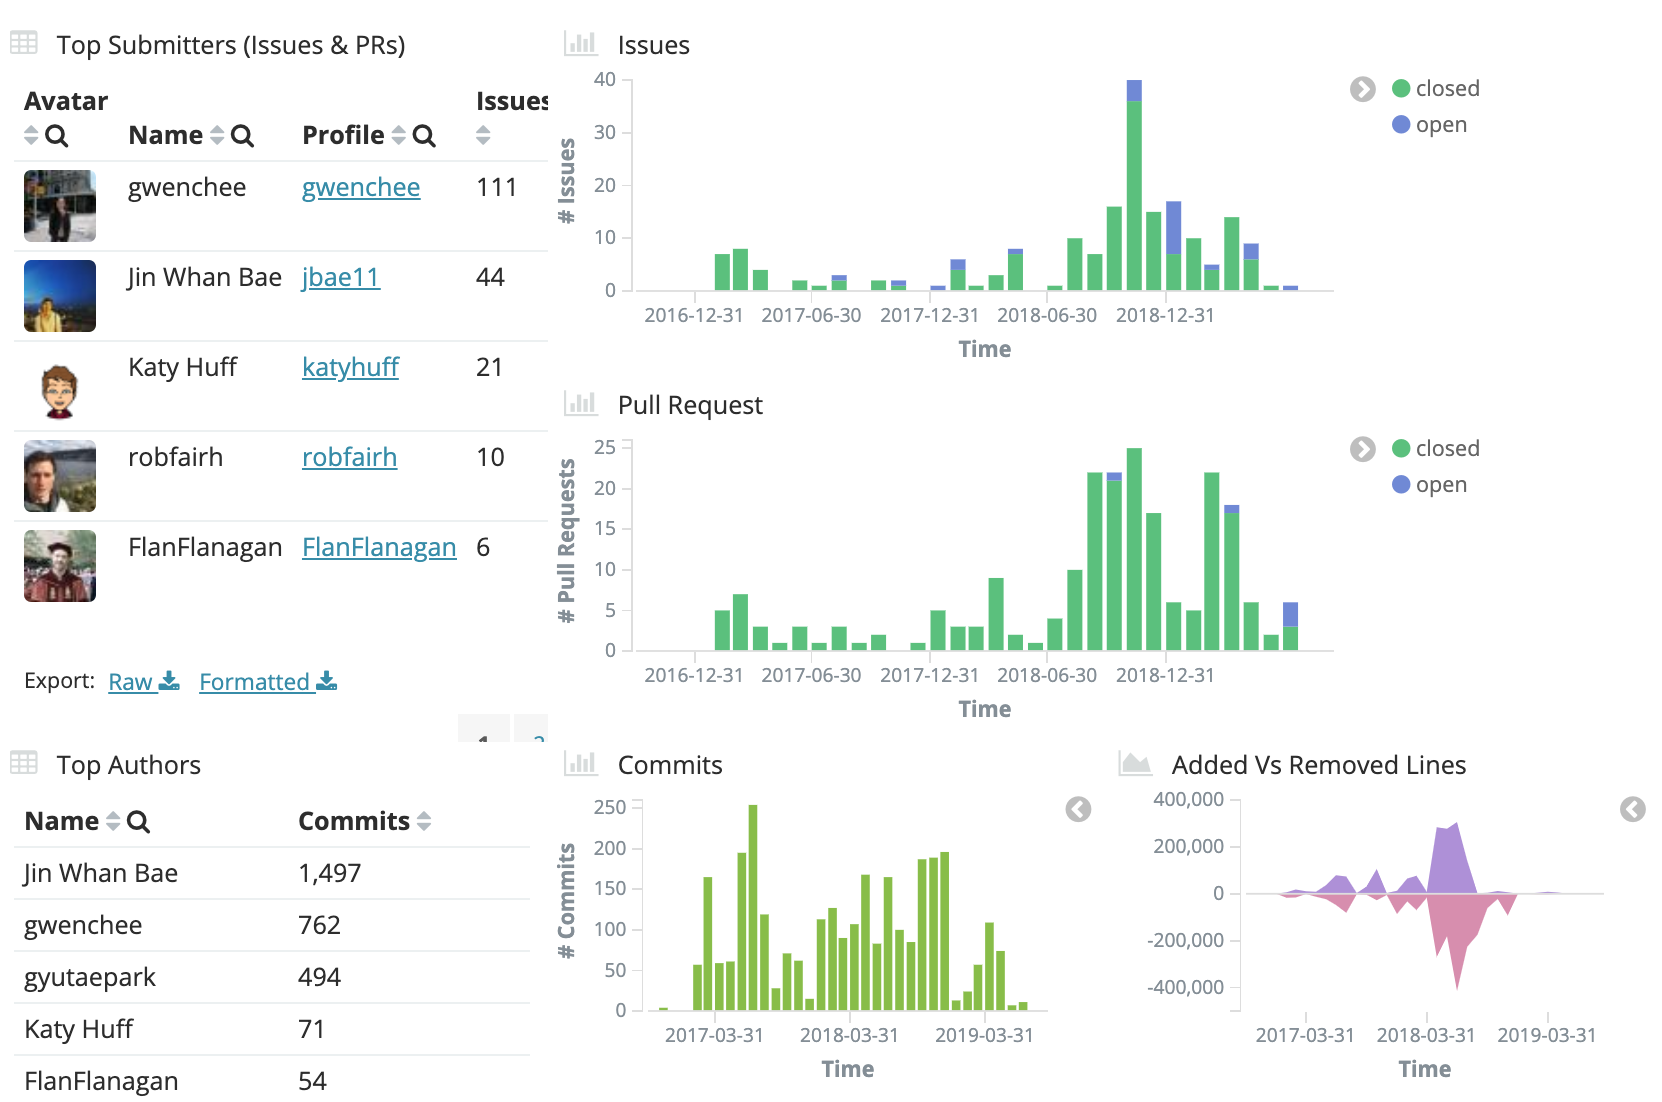
\includegraphics[width=0.9\textwidth]{images/git-stats-issues-ddca.png}
        \end{center}
              \caption{GitHub issues associated directly with this work.}
      \end{figure}
\end{frame}


\begin{frame}
        \frametitle{Quick Statistics}
    \begin{figure}[htbp!]
        \begin{center}
          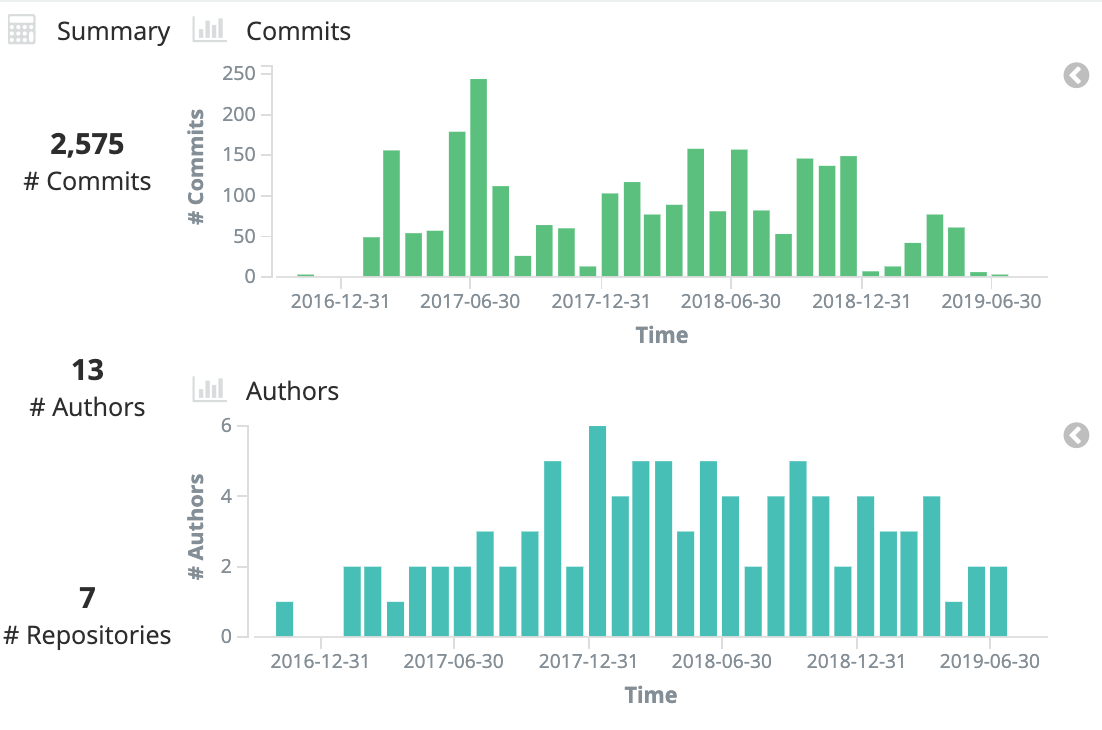
\includegraphics[width=0.9\textwidth]{images/git-stats-commits-ddca.png}
        \end{center}
              \caption{GitHub commits associated directly with this work.}
      \end{figure}
\end{frame}


\begin{frame}
        \frametitle{Quick Statistics}
    \begin{figure}[htbp!]
        \begin{center}
          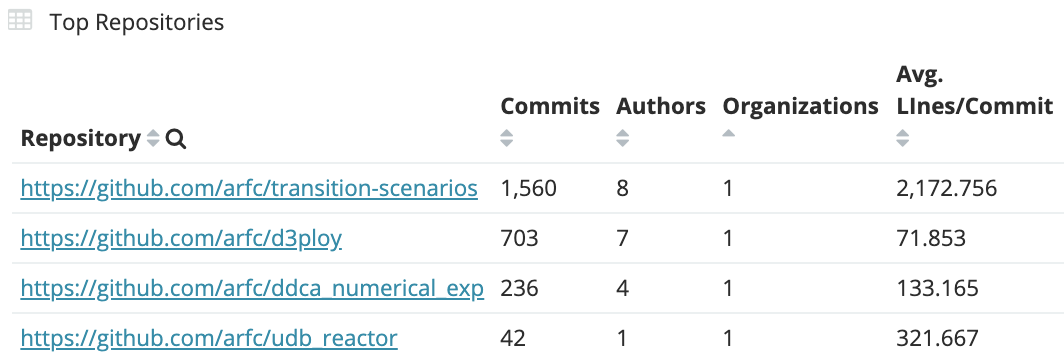
\includegraphics[width=\textwidth]{images/git-stats-lines-ddca.png}
        \end{center}
              \caption{Lines of code associated directly with this work.}
      \end{figure}
\end{frame}


\begin{frame}
        \frametitle{Detailed Schedule}
\begin{block}{2016}
        \begin{itemize}
       \item[$\checkmark$] Literature review of appropriate predictive algorithms.
       \item[$\checkmark$] Add stop and restart capabilities to Cyclus (bonus: HPC deployment addition).
        \end{itemize}
\end{block}
\begin{block}{2017}
        \begin{itemize}
       \item[$\checkmark$] Identify and rectify non-algorithmic capability gaps (e.g. specific fuel cycle process archetypes) necessary for transition simulation.
       \item[$\checkmark$] Create d3ploy
       \item[$\checkmark$] Add toolkit additions related for geospatial information
       \item[$\checkmark$] Implement non-optimizing (NO) methods in d3ploy.
        \end{itemize}
\end{block}
\end{frame}


\begin{frame}
        \frametitle{Detailed Schedule}
\begin{block}{2018}
        \begin{itemize}
       \item[$\checkmark$] Design numerical experiments (tests) for verifying Deterministic-Optimizing (DO) algorithms in the context of key transitions.
       \item[$\checkmark$] Implement Deterministic Optimizing (DO) methods in d3ploy.
       \item[$\checkmark$] Design numerical experiments (test) for verifying Stochastic-Optimizing (SO) algorithms in the context of key transitions. 
        \end{itemize}
\end{block}
\begin{block}{2019}
        \begin{itemize}
       \item[$\checkmark$] Implement Stochastic Optimizing (SO) methods in d3ploy.
       \item[$\checkmark$] Add additional capabilities to the predictive methods. (Buffers, reprocessing complexity handing)
       \item[$\checkmark$] Demonstrate and compare the new capability in the context of the evaluation groups the EG 23, 24, 29, 30
        \end{itemize}
\end{block}
\end{frame}


\begin{frame}
        \frametitle{Detailed Schedule}
    \begin{figure}[htbp!]
        \begin{center}
          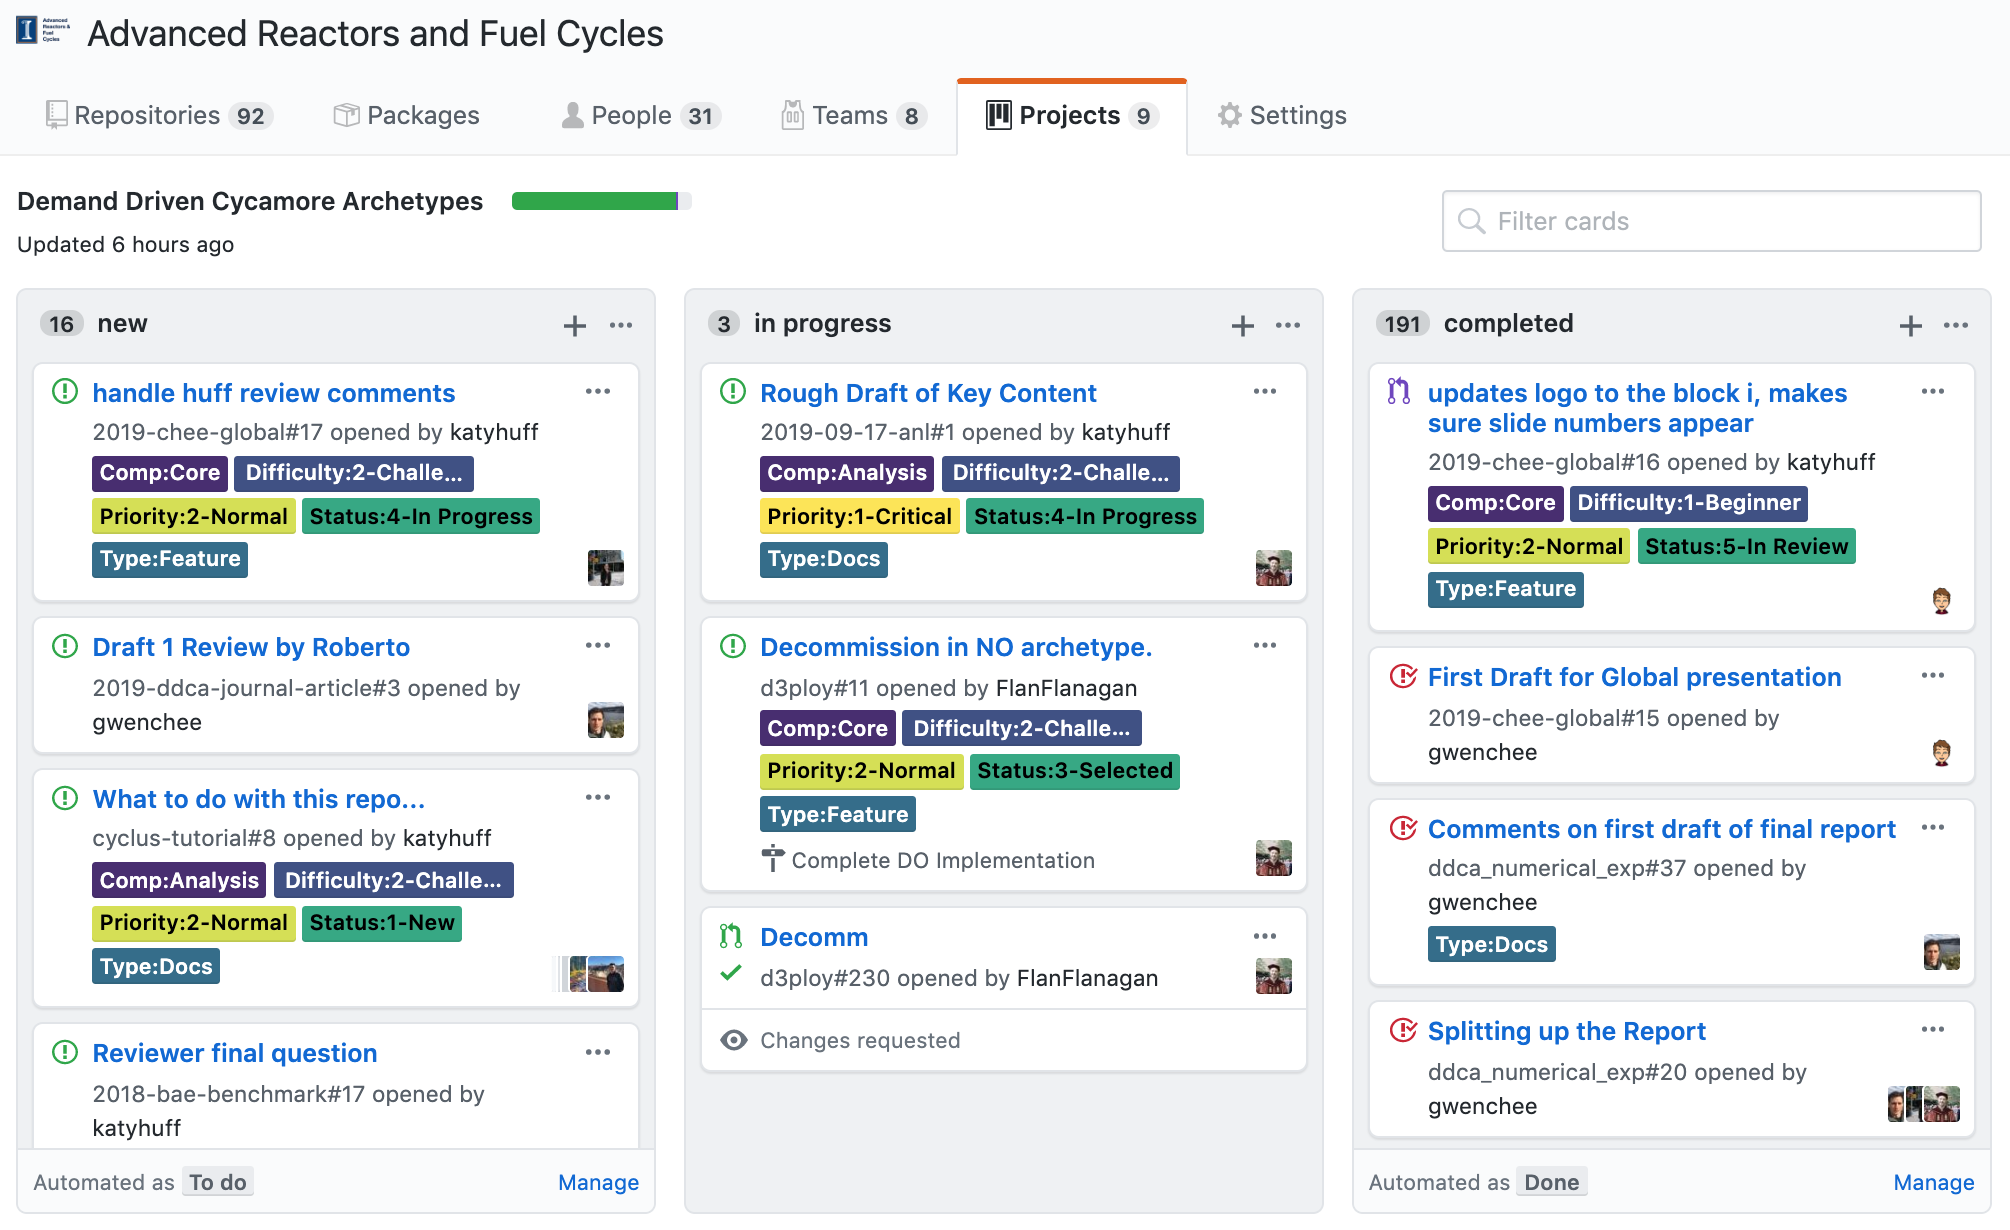
\includegraphics[width=\textwidth]{images/github-ddca-proj.png}
        \end{center}
              \caption{Project management associated with this project.}
      \end{figure}
\end{frame}

